\label{Chapter5} % Change X to a consecutive number; for referencing this chapter elsewhere, use \ref{ChapterX}
\chapter{扩展方案} % Main chapter title
\section{目标问题}
上述提到给予RISC-V中PMP设计的KeyStone存在PMP寄存器不足的问题,
如(图~\ref{fig:pmpcfg}), 在RV64的模式下有2个pmpcfg寄存器pmpcfg0和pmpcfg2,
包含了可以指明解析方案的16个8个bits组成的pmpxcfg寄存器,即pmp0cfg-pmp15cfg。
在一些场景下仅仅这16个权限寄存器可能并不足够。为了在不改变原始硬件的情况下,
增加可用的PMP寄存器范围,可以给出PMP寄存器的扩展方案。

\begin{figure}
    \centering
    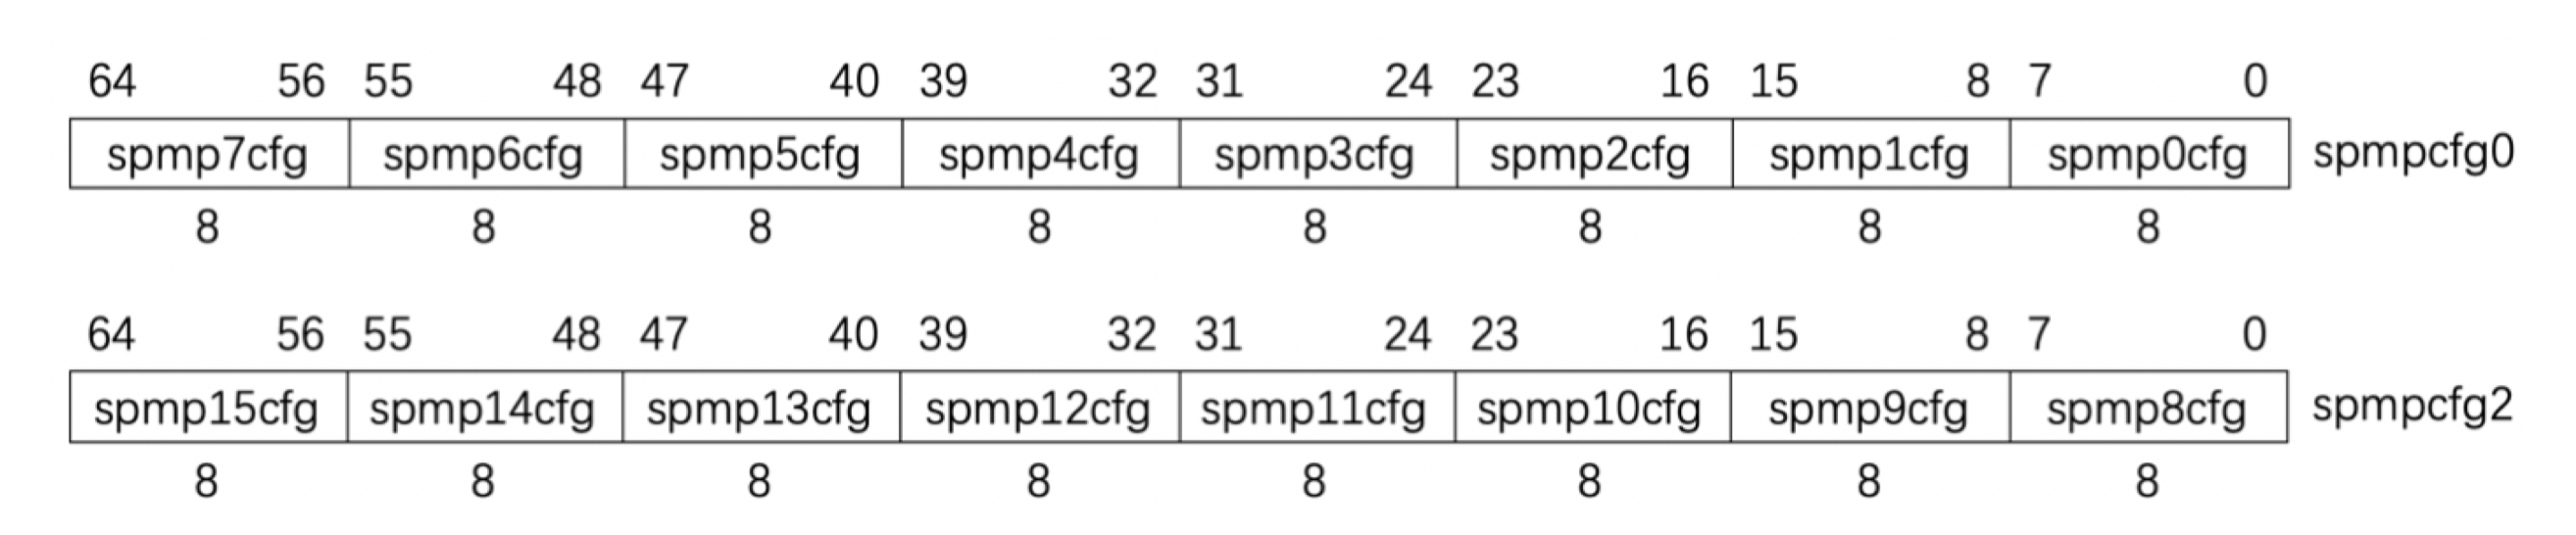
\includegraphics[scale=0.30]{Figures/extend/pmpcfg.png}
    \decoRule
    \caption{pmpcfg寄存器}
    \label{fig:pmpcfg}
\end{figure}

\begin{figure}
    \centering
    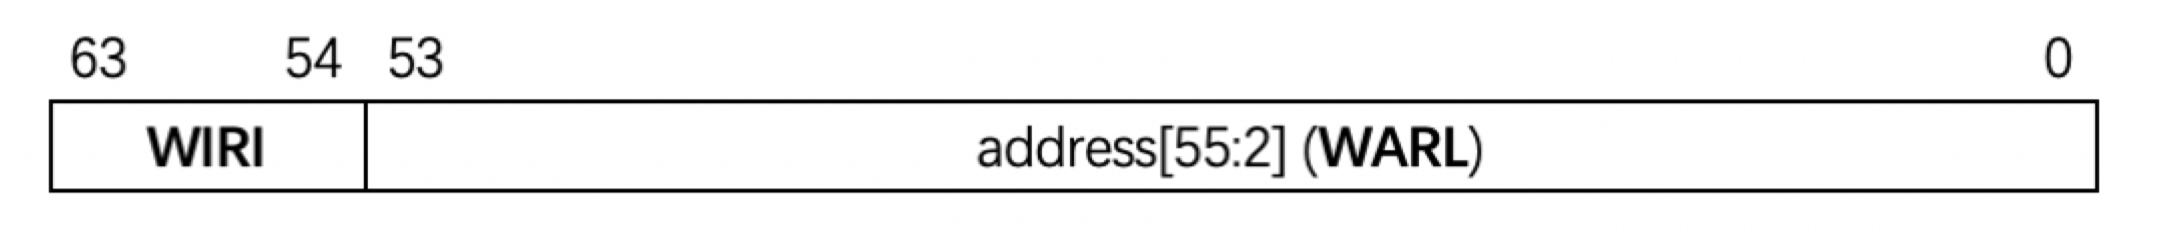
\includegraphics[scale=0.30]{Figures/extend/addrformat.png}
    \decoRule
    \caption{地址寄存器格式}
    \label{fig:addrformat}
\end{figure}

\section{扩展思路}
原始的PMP是通过Monitor来配置Machine Code用来保护Monitor最基本的物理地址空间。其本来的
RISC-V硬件线程(hart)的特权等级如(图~\ref{fig:level})所示
为了扩大保护的范围,可以考虑当一个Kernel已经进入了由PMP寄存器保护的物理内存之后,即附属在一个hart上后,
可以借用原来的寄存器在Kernel层再做一次映射,以此从物理上在同一个kernel中隔离更多的空间。
当一个用户端的App从U状态下进行向下寻址后,
可以先由PMA检查和原始PMP检查对其进行校验,在通过之后,可以再使用Kernel层上的扩展隔离,
以此达到进一步划分物理空间和App所属的地址隔离问题,CFG基址寄存器如(图~\ref{fig:addrformat})。

\begin{figure}
    \centering
    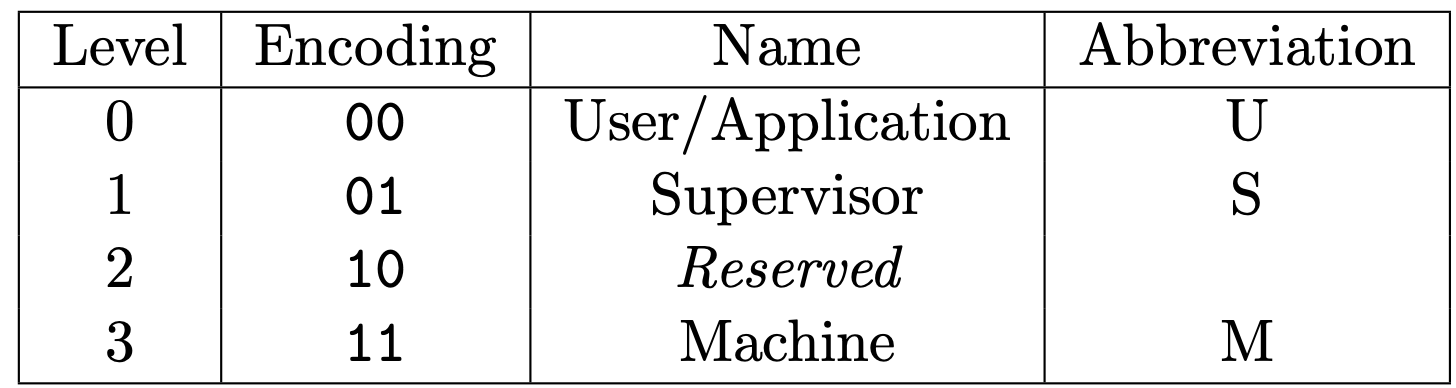
\includegraphics[scale=0.30]{Figures/extend/level.png}
    \decoRule
    \caption{硬件线程特权等级}
    \label{fig:level}
\end{figure}

\subsection{实际扩展}
具体的扩展方案,可以通过一个线程在某一Kernel由PMP分配的物理空间之后,即hart运行在U模式下时,
可以将PMP寄存器进行重置和复用,可以通过U模式下重置,可以在U模式下用和PMP相同的策略进一步划分内存。
首先hart进入S模式,Machine Code将原始PMP寄存器的值保存至Security Monitor中,
之后使用Kernel自己的策略重置PMP寄存器,进行地址的划分和隔离。
当离开U模式时,Machine Code也会恢复原来存储在Security Monitor中的寄存器的值。



\subsection{扩展格式}
在U模式下的扩展采用原有PMP的隔离策略,并在异常等方面做降级处理。
仍然采用如(图~\ref{fig:pmpcfg})的方式,使用pmpcfg0和pmpfcg2寄存器存储pmp0cfg到pmp15cfg的值,来划分权限,
使用PMP地址寄存器来存储地址划分的基础地址。
CFG的格式和原始PMP积寄存器CFG基本一致,如(图~\ref{fig:cfgformat}),X位,W位和R位分别表示可读可写和可执行的权限。
A位表示寻址策略,如(图~\ref{fig:afield})所示,当A的值为0时,表示此扩展禁用不匹配任何地址。当A=1时采用TOR分配到地址空间的上界。
当A=2时采用NA4策略,分配4byte对齐的空间。
当A=3时采用NAPOT策略,即分配一个对其且大小为2的整数幂的空间,在这种模式下最小分配地址为8bytes。
划分地址空间的结果如(图~\ref{fig:address})
L位代表着对新的PMP扩展进行上锁。以上的权限只在U模式下生效,原来的M模式仍然可以正常的访问内存,
且可以重置和解锁扩展PMP的L位。
\begin{figure}
    \centering
    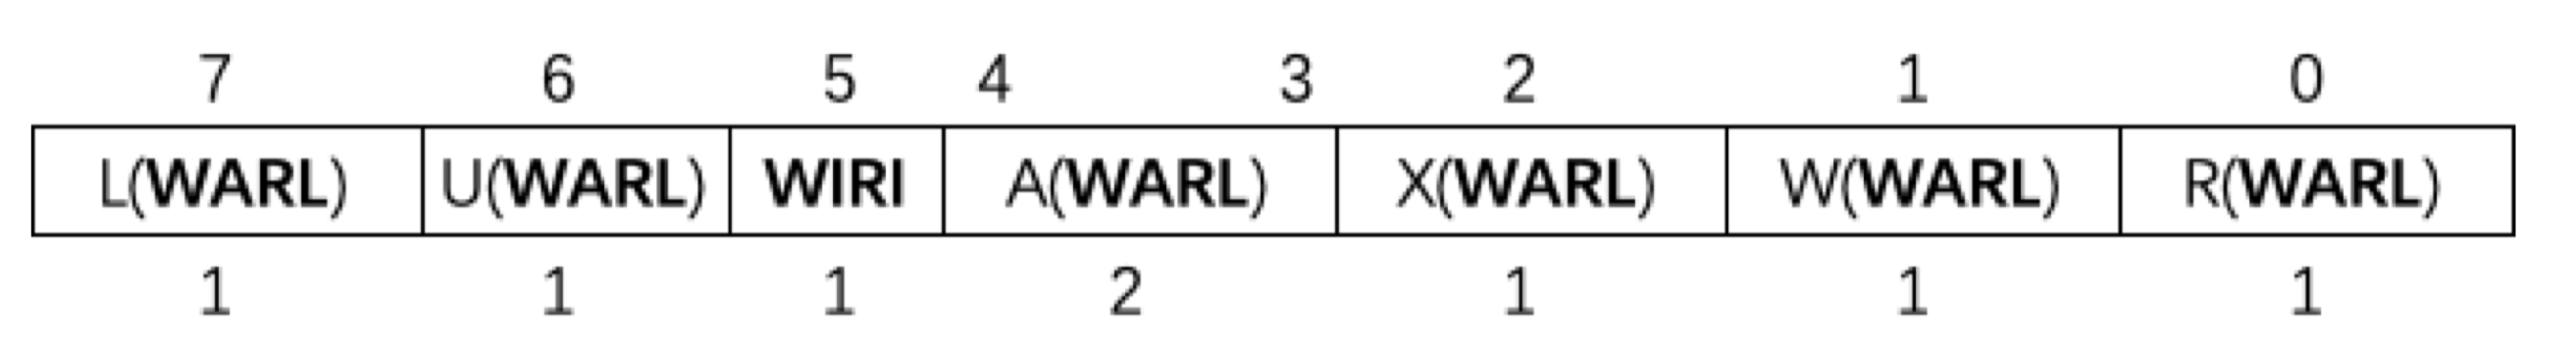
\includegraphics[scale=0.30]{Figures/extend/cfgformat.png}
    \decoRule
    \caption{CFG格式}
    \label{fig:cfgformat}
\end{figure}
\begin{figure}
    \centering
    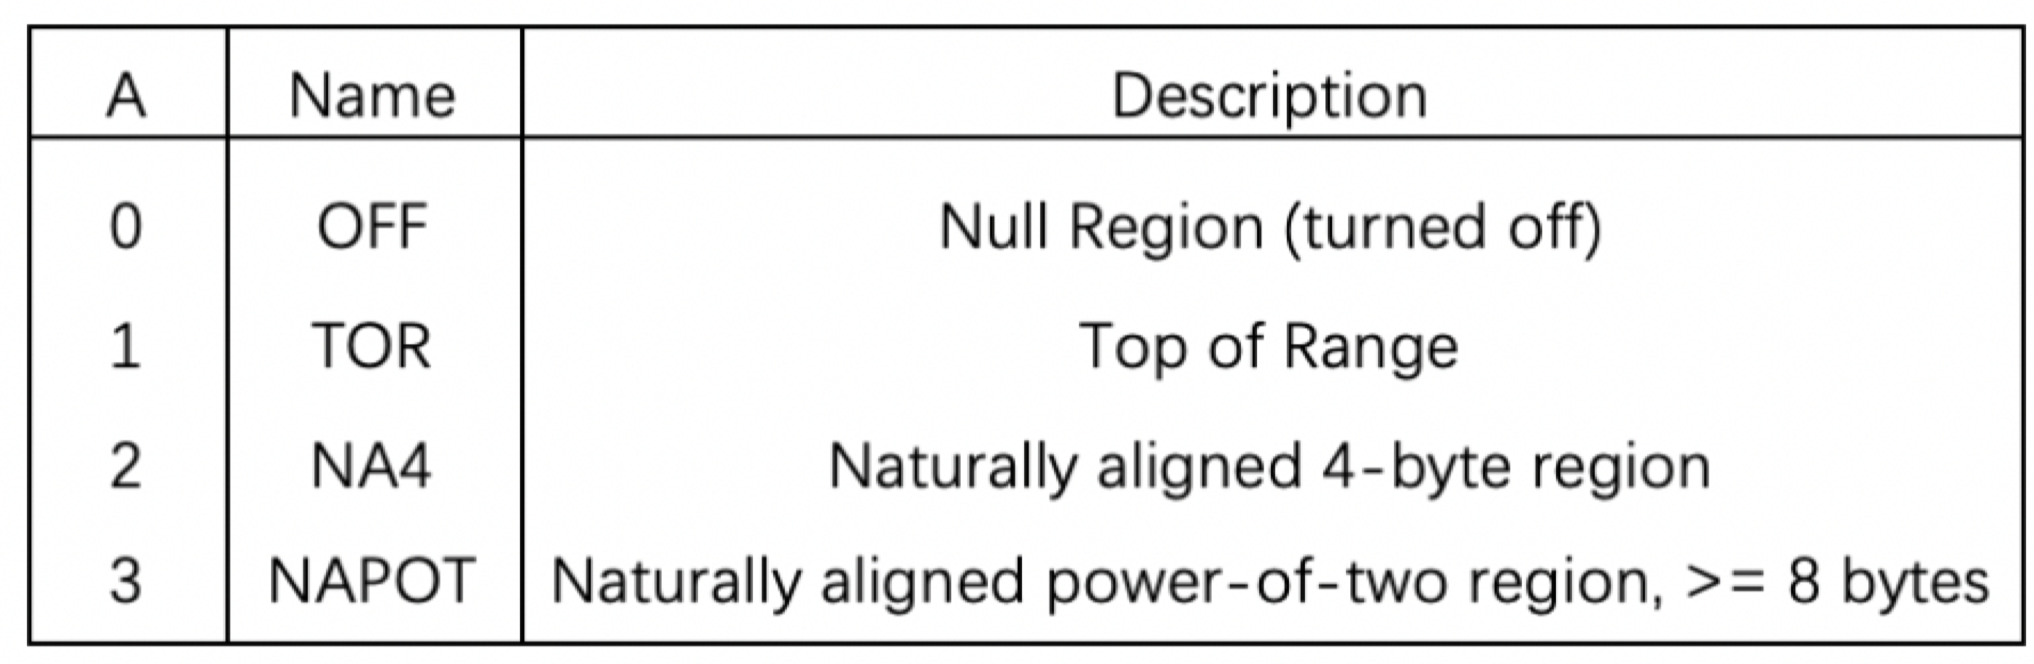
\includegraphics[scale=0.35]{Figures/extend/afield.png}
    \decoRule
    \caption{A位取值}
    \label{fig:afield}
\end{figure}

\subsection{权限和异常}
扩展的PMP只会在寻址已经通过了原来PMP的检查之后才会进行。
原始的PMP会通过最低位表示一次访问存储的成功或者失败。
首先PMP会检测其访问的地址是否在访问范围内,如果在不在访问范围内,则直接将结果设置为失败。
若在访问范围内,则根据实际的读写执行权限进行判定。
若访问失败,则会出现一个指令访问异常。
和原始PMP类似扩展的PMP也使用最低位来表示访存的失败,在原来PMP的检查之后,U模式下仍然会先检查方寸是否在扩展PMP规定的范围内,
这次检查相比于原始PMP的检查具有更细的粒度。在检查通过之后,仍然会根据读写执行权限进行判定,
若访问失败,会产生出一个页错误,这个错误可以交给U模式下kernel自己处理,也可以让更高层的Machine Code进行处理。


\section{场景分析}
本章节将分析上面的扩在实际应用场景的中的表现,筛选出上述扩展最适合的场景和最不适合的场景。
上述扩展的优势在于将原本数量较少的PMP寄存器进行了扩展,将16哥用于隔离的寄存器扩大位256个,极大提高了物理空间的隔离能力。
同时在IOT场景下,有些设备和系统不支持基于页的虚存管理,因此在S模式下的隔离将变得十分困难。而上述扩展提供了一种
在U模式下直接在hart上进行物理隔离的新方案。

\begin{figure}
    \centering
    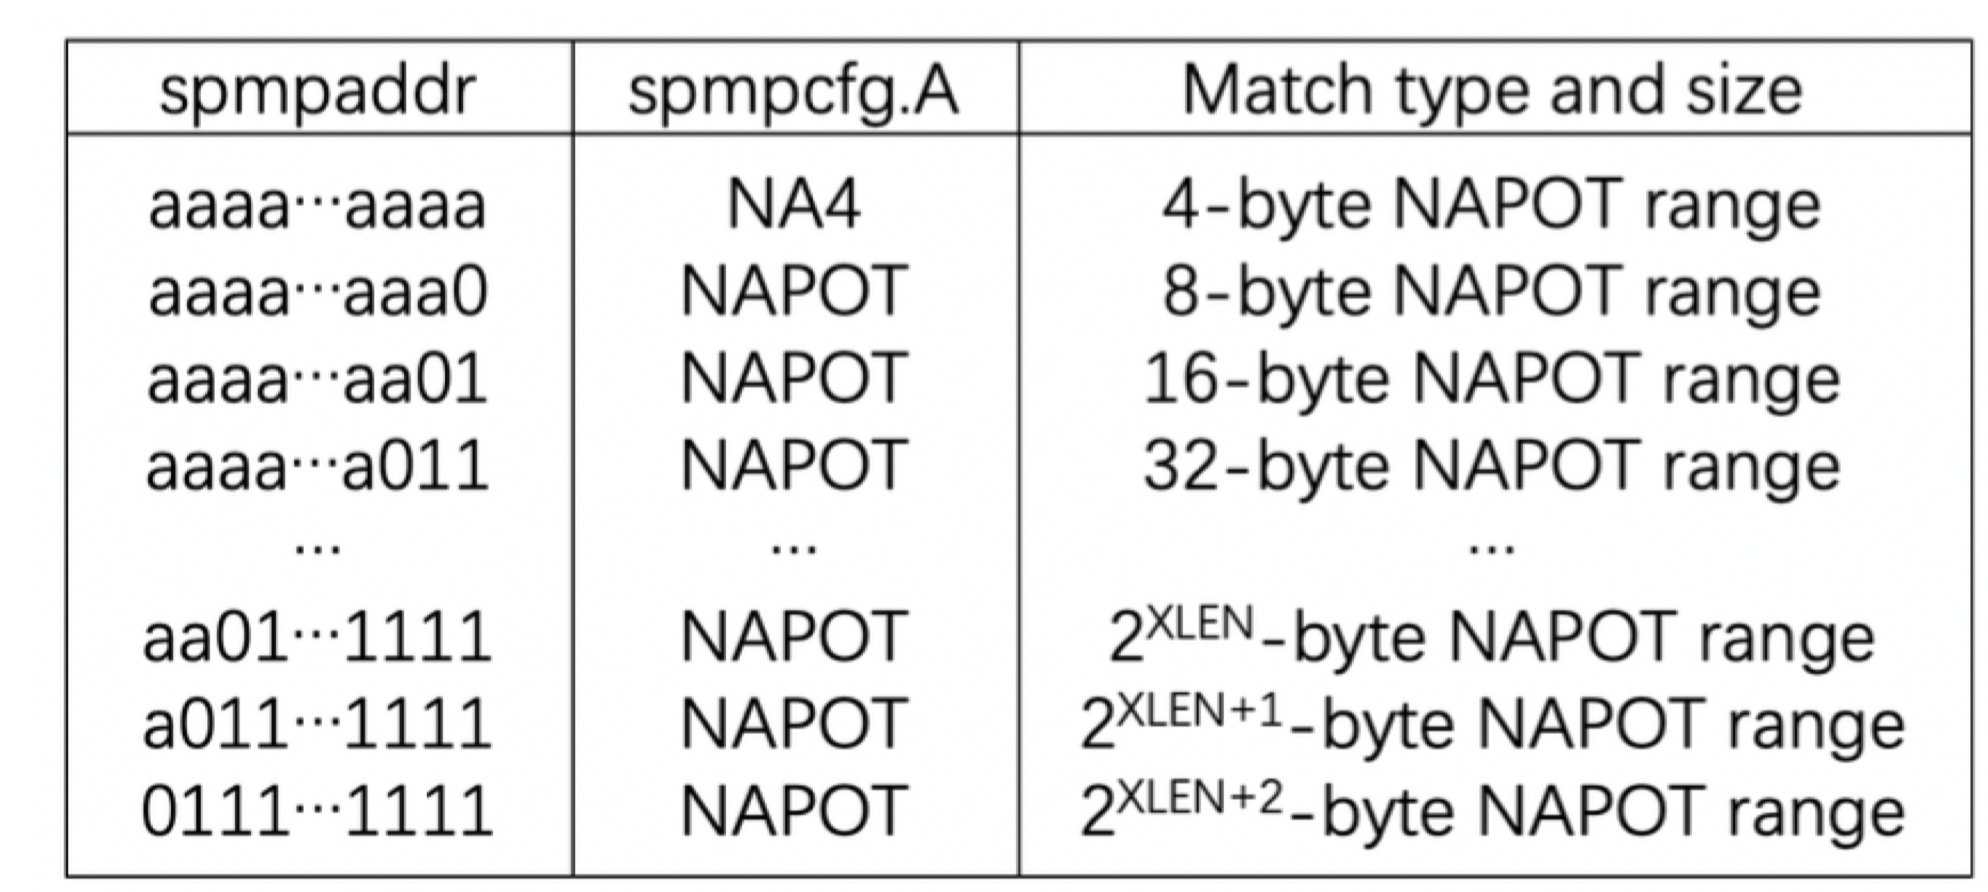
\includegraphics[scale=0.35]{Figures/extend/address.png}
    \decoRule
    \caption{地址空间划分}
    \label{fig:address}
\end{figure}

\subsection{适用场景}
我们认为上述扩展非常适合一个车载系统场景。车载系统中需要支持多个IOT设备,上述系统可以有效解决其IOT设备仅用PMP,没有页表,隔离性不足的问题。
同时在运行时需要更多的App层应用,其同时需要隔离的应用可能超过16个,上述扩展可以对车载系统上进行更好的隔离。
划分地址空间的结果如(图~\ref{fig:car})所示,我们给出了一个简易的车载系统可能应用分布。


可以看到最下面绿色部分是由Machine Code保障安全的Security Monitor, 
上面黄色部分是S模式下对原来的PMP进行再扩展。
最上面白色部分是U模式下运行车载系统相关应用程序。

首先像制动模块这样与安全相关的部分,应该与其他应用从硬件上进行个隔离。其次像制冷这类需要主要操控硬件的模块也应该由PMP进行隔离,
如果以后为制冷模块增加更智能的交互设计,如温度感知等,其余应用可以在PMP划分的制冷模块的基础上进一步使用上述PMP扩展划分,划分出温度感知,
自动调节,制冷只热,以及车窗去雾等应用。最后像一些借助信号的通讯模块,其实时性和安全性相比前其他模块的较弱,可以放在一个由PMP隔离的物理空间下
对于其内部的诸多U模式应用,即可以采用PMP扩展的隔离。

对于该场景,可以显示出此扩展的必要性和有效,
如果全部采用PMP隔离,会发现由于PMP寄存器有限,只有16个,不足以隔离数量较多的车载应用。
而如果使用部分隔离部分不隔离的方案,不隔离的部分则具有很高的被入侵的风险性。
同时很多车载IOT设备不支持页表,基本的操作系统层面的隔离也不能支持。
其系统安全危险性高。因此需要使用PMP扩展来解决上述遇到的问题。
\begin{figure}
    \centering
    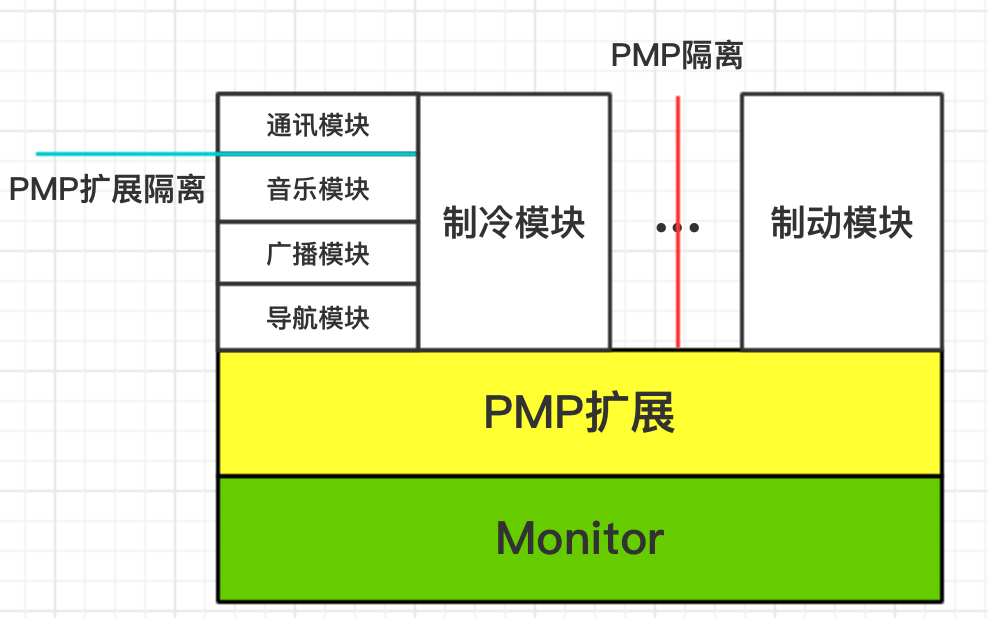
\includegraphics[scale=0.45]{Figures/extend/car.png}
    \decoRule
    \caption{车载系统示意图}
    \label{fig:car}
\end{figure}

\subsection{不适用场景}
我们认为这种扩展并没有特别不适合的场景,因为其根本思想是对原来RISC-V的一个扩展。
只能说在应用数量不是特别庞大,原有PMP寄存器完全足够使用的情况下,使用原来的PMP设计可以
避免使用扩展设计带来的额外的开销,又能保证其基本的隔离性。

其次随着硬件的不断发展,在以后这样的从软件层面的扩展设计可能会被新的硬件取代。
随着硬件的发展和迭代,其可以更高效的解决软件扩展性能开销的问题。

\section{小结}
本章节从上一章节最后对与基于RISC-V架构的PMP方案现存问题出发,通过PMP在U模式下的扩展隔离设计。
将原本16个PMP寄存器扩展为16个,解决了在IoT场景中,没有页表情况下,只有PMP隔离不充分的问题,以及
原本PMP寄存器数量不足的问题。之后借助原来PMP的设计解释了PMP扩展设计的思想。最后给出来一个适合该
扩展设计的使用场景,并加以分析。对于不适用的场景则给出来了简单的分析和总结。